\section{Le groupe \texorpdfstring{$SL_2(\Z)$}{SL2(Z)}}

\[ SL_2(\Z) = \{ M \in \mathscr M_2(\Z) \mid \det M = 1 \} \quad \text{groupe pour } \times \]

But : trouver un ou plusieurs systèmes de générateurs.

\uindent{Action de $SL_2(\Z)$ sur $\Z^2$} $\begin{pmatrix} a & b \\ c & d \end{pmatrix} \in SL_2(\Z)$

\[
    \begin{pmatrix} a & b \\ c & d \end{pmatrix} \begin{pmatrix} n \\ m \end{pmatrix} = \begin{pmatrix} an+bm \\ cn+dm \end{pmatrix} \in \Z^2
\]

\[ [n, m] = \left\{ M \begin{pmatrix} n \\ m \end{pmatrix} \mid M \in SL_2(\Z) \right\} = \text{orbite de } \begin{pmatrix} n \\ m \end{pmatrix} \]

\uindent{Cas $n^{\circ}1$} $n \wedge m = 1$, alors $\exists a, b$, $an + bm = 1$ $(= (a-km)n + (b+kn)m)$

\[
    M = \begin{pmatrix} a & b \\ a-m & b+n \end{pmatrix} \quad \det = ab + an - ab + mb = 1
\]
\[
    \text{donc } [n, m] = [1, 1] \quad (\sim \text{orbite})
\]

\[
    M \begin{pmatrix} n \\ m \end{pmatrix} = \begin{pmatrix} 1 \\ 1 \end{pmatrix}
\]

\uindent{Réciproquement} si $[n, m] = [1, 1]$, $\exists \begin{pmatrix} a & b \\ c & d \end{pmatrix} \in SL_2(\Z)$.

\[
    \begin{pmatrix} a & b \\ c & d \end{pmatrix} \begin{pmatrix} n \\ m \end{pmatrix} = \begin{pmatrix} 1 \\ 1 \end{pmatrix} \quad an + bm = 1 \quad \text{donc } n \wedge m = 1
\]

\[ [n, m] = [1, 1] \iff n \wedge m = 1 \]

Si $d = n \wedge m$, $n = d n'$ et $m = d m'$, $\exists M \in SL_2(\Z)$,

\[
    M \begin{pmatrix} n' \\ m' \end{pmatrix} = \begin{pmatrix} 1 \\ 1 \end{pmatrix} \text{ et donc } M \begin{pmatrix} n \\ m \end{pmatrix} = \begin{pmatrix} d \\ d \end{pmatrix} \quad \text{donc } [n, m] = [d, d]
\]

\[
    \text{Stabilisateur de } \begin{pmatrix} 1 \\ 0 \end{pmatrix} = \left\{ M \in SL_2(\Z) \mid M \begin{pmatrix} 1 \\ 0 \end{pmatrix} = \begin{pmatrix} 1 \\ 0 \end{pmatrix} \right\} = \left\{ \begin{pmatrix} 1 & n \\ 0 & 1 \end{pmatrix}, n \in \Z \right\}
\]
\begin{center}
    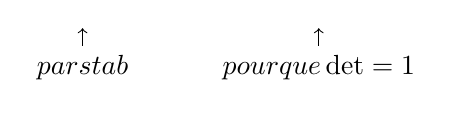
\begin{tikzpicture}
        \node (A) at (0,0) {$\text{par stab}$};
        \node (B) at (3,0) {$\text{pour que } \det=1$};
        \draw[->] (A) -- (0, 0.5);
        \draw[->] (B) -- (3, 0.5);
    \end{tikzpicture}
\end{center}

\[ T = \begin{pmatrix} 1 & 1 \\ 0 & 1 \end{pmatrix} \quad \forall n \in \Z, \, T^n = \begin{pmatrix} 1 & n \\ 0 & 1 \end{pmatrix} \]

\[ \implies \text{Stab de } \begin{pmatrix} 1 \\ 0 \end{pmatrix} = \{ T^n \mid n \in \Z \} = \langle T \rangle. \]

% \restaurergeometrie

\begin{theoreme}{}{}
    $SL_2(\Z)$ est engendré par $T = \begin{pmatrix} 1 & 1 \\ 0 & 1 \end{pmatrix}$ et $S = \begin{pmatrix} 0 & -1 \\ 1 & 0 \end{pmatrix}$.
\end{theoreme}

\begin{proof}
    Soit $M \in SL_2(\Z)$, et soit $\begin{pmatrix} n \\ m \end{pmatrix} = M \begin{pmatrix} 1 \\ 0 \end{pmatrix}$ la $1^{\text{ère}}$ colonne de $M$. \\
    $n \wedge m = 1$.

    \uindent{Affirmation} $\exists N \in \langle T, S \rangle$ tq $\begin{pmatrix} n \\ m \end{pmatrix} = N \begin{pmatrix} 1 \\ 0 \end{pmatrix}$.

    Supposons cette affirmation démontrée : $N \begin{pmatrix} 1 \\ 0 \end{pmatrix} = M \begin{pmatrix} 1 \\ 0 \end{pmatrix}$. \\
    $N^{-1} M \in \text{Stab} \begin{pmatrix} 1 \\ 0 \end{pmatrix} = \langle T \rangle$. \\
    $M = N \times T^k \in \langle S, T \rangle$. \\
    $\in \langle S, T \rangle$.

    \begin{proof}
    \uline{Démo de l'affirmation} : Si $|m| > |n|$, $S \begin{pmatrix} n \\ m \end{pmatrix} = \begin{pmatrix} -m \\ n \end{pmatrix}$, $|m| > |n|$. \\
    On peut supposer $|n| > |m|$.
    \begin{align*}
        n &= m q_1 + r_1 \qquad \text{\reflectbox{$\hookrightarrow$} algo d'Euclide} \\
        m &= r_1 q_2 + r_2 \\
        & \dots \\
        r_{k-1} &= r_k q_{k+1} + r_{k+1}
    \end{align*}

    Dernier reste non nul $= \pgcd = 1$.

    \uline{Interprétation matricielle} :
    \begin{align*}
        \begin{pmatrix} n \\ m \end{pmatrix} &= \begin{pmatrix} 1 & q_1 \\ 0 & 1 \end{pmatrix} \begin{pmatrix} r_1 \\ m \end{pmatrix} = T^{q_1} \begin{pmatrix} r_1 \\ m \end{pmatrix} \\
        &= T^{q_1} S \begin{pmatrix} -m \\ r_1 \end{pmatrix} \quad \text{puis utilise ligne 2 algo d'Euclide} \\
        &= \begin{pmatrix} 1 & -q_2 \\ 0 & 1 \end{pmatrix} \begin{pmatrix} -r_2 \\ r_1 \end{pmatrix} = T^{-q_2} \begin{pmatrix} -r_2 \\ r_1 \end{pmatrix}
    \end{align*}
    On itère le processus jusqu'à obtenir le vecteur $\begin{pmatrix} \pm 1 \\ 0 \end{pmatrix}$ ou $\begin{pmatrix} 0 \\ \pm 1 \end{pmatrix}$, ce qui permet de conclure.
\end{proof}

\begin{align*}
    &= T^{-q_2} S \begin{pmatrix} -r_1 \\ -r_2 \end{pmatrix} \\
    & \vdots \\
    &= T^{\dots} S \begin{pmatrix} \pm 1 \\ 0 \end{pmatrix}
\end{align*}

Donc $\begin{pmatrix} n \\ m \end{pmatrix} \sim N \begin{pmatrix} 1 \\ 0 \end{pmatrix} \dots$ fin de la preuve.
\end{proof}

\begin{remarque}
    $ST = \begin{pmatrix} 0 & -1 \\ 1 & 0 \end{pmatrix} \begin{pmatrix} 1 & 1 \\ 0 & 1 \end{pmatrix} = \begin{pmatrix} 0 & -1 \\ 1 & 1 \end{pmatrix} = R$.
    \[ \langle S, T \rangle = \langle S, R \rangle = SL_2(\Z) \]
    Matrices d'ordre fini : $S^4 = I_2$ et $R^6 = I_2$.
\end{remarque}

Soit $\rho : SL_2(\Z) \to (\C^*, \times)$ un morphisme de groupes. \\
\uindent{Affirmation} $\Im \rho \subset \mathbb{U}_{12} \implies$ optimal, $\exists \rho, \Im \rho = \mathbb{U}_{12}$.

\begin{proof}
    $\Im \rho = \langle \rho(S), \rho(R) \rangle$. $\rho(S)^4 = \rho(S^4) = 1$ et $\rho(R)^6 = \rho(R^6) = 1$. \\
    $\rho(S), \rho(R) \in \mathbb{U}_{12}$.
\end{proof}

\uindent{Aff} 
\begin{itemize}
    \item $\forall n \geqslant 3$, le morphisme $SL_n(\Z) \to \C^*$ est trivial.
    \item Le morphisme de $SL_2(\Z) \to G$ abélien est trivial.
\end{itemize}

Soit $U = \begin{pmatrix} 1 & 0 \\ 1 & 1 \end{pmatrix}$. $U = TST$ donc $S = T^{-1} U T^{-1}$.

Donc $SL_2(\Z) = \langle T, U \rangle$. \\
$\hookrightarrow$ ordre infini (contrairement à $S$ et $R$).

\begin{theoreme}{}{}
    Soit $N \in \N^*$ dans $SL_2(\Z) \to SL_2(\Z/N\Z)$ \\
    $M \mapsto \overline{M}$ \\
    est un morphisme de groupes surjectif.
\end{theoreme}


Conséquence : $SL_2(\Z/N\Z)$ est un groupe engendré par 
\begin{itemize}
    \item $\bar U, \bar T$
    \item ordre fini égal à $N$.
\end{itemize}

\uindent{Exo} $N = 2^n$. $SL_2(\Z/2^n\Z) = \langle \bar U, \bar T \rangle$, ordre $2^n$.
\[ \forall M \in SL_2(\Z/2^n\Z), \text{ ordre } M \leqslant 3 \times 2^{n-1} \]

\[ SL_2(\Z) \to SL_2(\Z/2\Z) = \left\{ \begin{pmatrix} 1 & 0 \\ 0 & 1 \end{pmatrix}, \begin{pmatrix} 1 & 1 \\ 0 & 1 \end{pmatrix}, \begin{pmatrix} 1 & 0 \\ 1 & 1 \end{pmatrix}, \dots \right\} \]
$\hookrightarrow$ cardinal 6. \\
Isomorphe à $S_3$ : groupe des permutations à 3 éléments.

\[ SL_2(\Z) \to S_3 \to \{-1, 1\} \quad \text{signature} \]

\begin{proof}[Preuve de la surjectivité]
    On veut montrer que $SL_2(\Z) \to SL_2(\Z/N\Z)$ est surjectif.

    Soit $\begin{pmatrix} a & b \\ c & d \end{pmatrix} \in SL_2(\Z/N\Z)$. Je choisis $a, b, c, d \in \Z$ tels que $\overline{\begin{pmatrix} a & b \\ c & d \end{pmatrix}} = M$.
    
    Alors $ad - bc = 1 + lN$.

    \uindent{Affirmation} $\exists k \in \N$ tel que $a \wedge (b+kN) = 1$.

    Supposons l'affirmation vraie, posons $b' = b + kN$, $\Delta' = ad - b'c$. \\
    $\exists u, v, \, au + b'v = 1$.
    
    \[ M = \begin{pmatrix} a & b' \\ c - v(1-\Delta') & d + u(1-\Delta') \end{pmatrix} \]
    
    Alors $\overline{M} = M$ (modulo $N$) car $1-\Delta' \equiv 0 \pmod N$, et $\det M = 1$.

    \lvspace
    \uline{Dém de l'aff} : Soit $p \in \mathbb{P}$ divisant $a$.
    \begin{itemize}
        \item Si $p \mid b$, $p \nmid N$ (sinon $\det \equiv 0 \pmod p$).
        \item Si $p \nmid b$, alors $p \nmid b+pN$.
    \end{itemize}
    $\to$ on prend $k = \prod_{\substack{p \in \mathcal P \\ p \mid a, p \nmid b}} p_i$.
    
    Vérification : ça fonctionne, $a \wedge (b+kN) = 1$.
\end{proof}